% Generated from the public primitive catalog. Original Atlas drawing; Apache-2.0.
% Target: sha3-256; view: detail
\documentclass[border=9pt]{standalone}
% Original Atlas figure theme. Apache-2.0; see the repository LICENSE.
\usepackage[T1]{fontenc}
\usepackage{lmodern}
\usepackage{amsmath,amssymb}
\usepackage{tikz}
\usetikzlibrary{arrows.meta,positioning,calc,fit,backgrounds,decorations.pathreplacing,matrix}
\definecolor{atlasInk}{HTML}{172235}
\definecolor{atlasTeal}{HTML}{0D7B7D}
\definecolor{atlasMuted}{HTML}{637278}
\definecolor{atlasFill}{HTML}{EAF4F2}
\definecolor{atlasLine}{HTML}{B6C8C7}
\tikzset{
  every picture/.style={line width=.65pt,draw=atlasInk,>=Latex},
  every node/.style={text=atlasInk,font=\sffamily\small},
  box/.style={draw,rounded corners=1.5pt,minimum height=.9cm,minimum width=1.6cm,align=center,inner sep=6pt,fill=white},
  accent/.style={box,draw=atlasTeal,fill=atlasFill},
  wire/.style={->,line width=.7pt},
  keywire/.style={wire,draw=atlasTeal,dashed},
  xor/.style={draw,circle,fill=white,inner sep=0pt,minimum size=.38cm},
  add/.style={draw,rectangle,fill=white,inner sep=0pt,minimum size=.38cm},
  note/.style={font=\sffamily\scriptsize,text=atlasMuted,align=center},
  phase/.style={font=\sffamily\small\bfseries,text=atlasTeal},
  group/.style={draw=atlasLine,dashed,rounded corners=2pt,inner sep=8pt}
}
\newcommand{\rotl}{\mathbin{\lll}}
\newcommand{\rotr}{\mathbin{\ggg}}
\newcommand{\kx}{\operatorname{Keccak}\!\text{-}\!f[1600]}

\newcommand{\AtlasKeyBits}{k}
\newcommand{\AtlasKeyWords}{N_k}
\newcommand{\AtlasRounds}{N_r}
\newcommand{\AtlasPriorRounds}{N_r-1}
\newcommand{\AtlasRoundKeys}{N_r+1}
\newcommand{\AtlasDoubleRounds}{N_r/2}
\newcommand{\AtlasSixRoundGroups}{N_r/6}
\newcommand{\AtlasFLGroups}{N_r/6-1}
\newcommand{\AtlasRoundStart}{24-n}
\newcommand{\AtlasBlockBits}{b}
\newcommand{\AtlasOutputBits}{256}
\newcommand{\AtlasStateBits}{1600}
\newcommand{\AtlasNonceBits}{v}
\newcommand{\AtlasCounterBits}{q}
\newcommand{\AtlasStreamBlockBits}{b}
\newcommand{\AtlasRate}{1088}
\newcommand{\AtlasCapacity}{512}
\newcommand{\AtlasSteps}{N}
\newcommand{\AtlasLastStep}{N-1}
\newcommand{\AtlasWordBits}{200}
\newcommand{\AtlasHashWords}{50}
\newcommand{\AtlasFeedForward}{\boxplus}
\newcommand{\AtlasByteOrder}{big-endian}
\newcommand{\AtlasDomain}{01}
\newif\ifAtlasXof
\AtlasXoffalse
\begin{document}
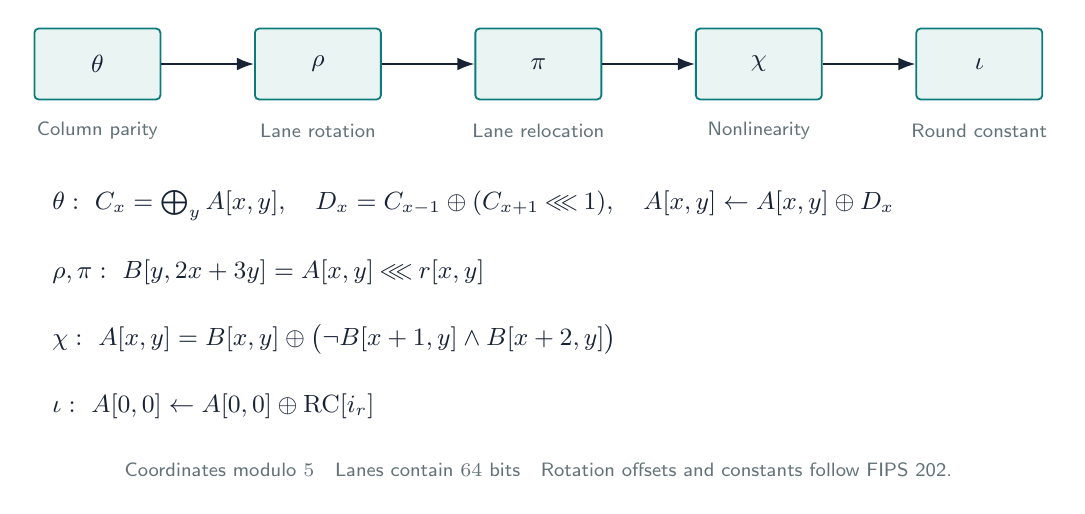
\begin{tikzpicture}
  \foreach \x/\name/\label in {0/theta/\theta,2.8/rho/\rho,5.6/pi/\pi,8.4/chi/\chi,11.2/iota/\iota} {
    \node[accent,minimum width=1.6cm] (\name) at (\x,1.5) {$\label$};
  }
  \draw[wire] (theta) -- (rho); \draw[wire] (rho) -- (pi);
  \draw[wire] (pi) -- (chi); \draw[wire] (chi) -- (iota);
  \node[note] at (0,.65) {Column parity}; \node[note] at (2.8,.65) {Lane rotation};
  \node[note] at (5.6,.65) {Lane relocation}; \node[note] at (8.4,.65) {Nonlinearity};
  \node[note] at (11.2,.65) {Round constant};
  \node[anchor=west] at (-.7,-.3) {$\theta:\ C_x=\bigoplus_y A[x,y],\quad D_x=C_{x-1}\oplus(C_{x+1}\rotl1),\quad A[x,y]\gets A[x,y]\oplus D_x$};
  \node[anchor=west] at (-.7,-1.15) {$\rho,\pi:\ B[y,2x+3y]=A[x,y]\rotl r[x,y]$};
  \node[anchor=west] at (-.7,-2) {$\chi:\ A[x,y]=B[x,y]\oplus\bigl(\neg B[x+1,y]\mathbin{\land}B[x+2,y]\bigr)$};
  \node[anchor=west] at (-.7,-2.85) {$\iota:\ A[0,0]\gets A[0,0]\oplus\mathrm{RC}[i_r]$};
  \node[note] at (5.6,-3.65) {Coordinates modulo $5$\quad Lanes contain $64$ bits\quad Rotation offsets and constants follow FIPS 202.};
\end{tikzpicture}

\end{document}
